% \section{Discussion of the uniqueness}\label{proof}
% \ligeng{TODO: format the notions.} \ligeng{Justify layer types.}

Let $X_\ell$ and $y_\ell$ be the input and output for $\ell^{th}$ layer. Given the weights $w_\ell$, the calculating process of inputs $X$ labels $Y$ can written as 

\begin{align*} 
    y_\ell &= f_\ell(X_\ell; w_\ell) \\
    % y_{\ell+1} &= f_{\ell + 1}(X_{\ell + 1}; w_{\ell + 1}) \\
    y &=   f_{N} ( f_{N-1} ( ... f_1 (X, w_1) ...w_{N-1} ) w_N) \\
      &= F(X, W)
\end{align*}

We care about the uniqueness between inputs $X, Y$ and gradients $\Delta W$. Is it possible that there is another pair of $X', Y'$ that produces the gradients that is same as previous?


\begin{equation}
    \frac{\partial Loss(F(X, W), Y)}{\partial W} = \frac{\partial Loss(F(X', W), Y')}{\partial W'} 
\end{equation}


Assume $j^{th}$ layer is a linear operation, for weight $w_j$

% $$
%     \frac{\partial Loss}{\partial w_{j}} = 
%     \frac{\partial Loss'}{\partial w_{j}}
% $$

\begin{equation}\label{eq:dldw_{j}}
    \frac{\partial Loss}{\partial y_{j}}
    \frac{\partial y_{j}}{\partial w_{j}}
    = 
    \frac{\partial Loss'}{\partial y'_{j}}
    \frac{\partial y'_{j}}{\partial w_{j}}
\end{equation}

For weight $w_{j-1}$

\begin{equation}\label{eq:dldw_{j-1}}
    \frac{\partial Loss}{\partial y_{j}}
    \frac{\partial y_{j}}{\partial y_{j-1}}
    \frac{\partial y_{j-1}}{\partial w_{j-1}}
    = 
    \frac{\partial Loss'}{\partial y'_{j}}
    \frac{\partial y'_{j}}{\partial y'_{j-1}}
    \frac{\partial y'_{j-1}}{\partial w'_{j-1}}
\end{equation}

Note, as $f_j()$ is a linear operation, $ \frac{\partial y_{j}}{\partial y_{j-1}}$ actually only relates with  $w_{j-1}$, regardless the inputs $ y_{j-1} $. The formula Eq.~\ref{eq:dldw_{j-1}} can be further simplified to 
 
\begin{equation}
    \frac{\partial Loss}{\partial y_{j}}
    % \frac{\partial y_{j}}{\partial y_{j-1}}
    \frac{\partial y_{j-1}}{\partial w_{j-1}}
    = 
    \frac{\partial Loss'}{\partial y'_{j}}
    % \frac{\partial y'_{j}}{\partial y'_{j-1}}
    \frac{\partial y'_{j-1}}{\partial w'_{j-1}}
\end{equation}

Substitute $\frac{\partial Loss}{\partial y_{j}}$ and $\frac{\partial Loss'}{\partial y_{j}}$ from Eq.~\ref{eq:dldw_{j}},

\begin{equation}
    x_{j} f_{j} (x_{j}, w_{j}) 
    =
    x'_{j} f_{j} (x'_{j}, w_{j}) 

\end{equation}

\zhijian{this part seems wrong....}

Since $f_j$ is a linear layer, $x_j f_j(x_j, w_j)$ is monotonous. When the equation holds, $ x_{j} $ must be equivalent as  $ x'_{j} $, which contradicts with the initial assumption $X \neq X, Y \neq Y'$.  
\newcommand\imgwidth{0.07}

% \section{Method}\label{sec:methods}

\section{Method}\label{sec:methods}

% \textbf{Problem Setup.} In 

\begin{figure}[t]
    \centering
    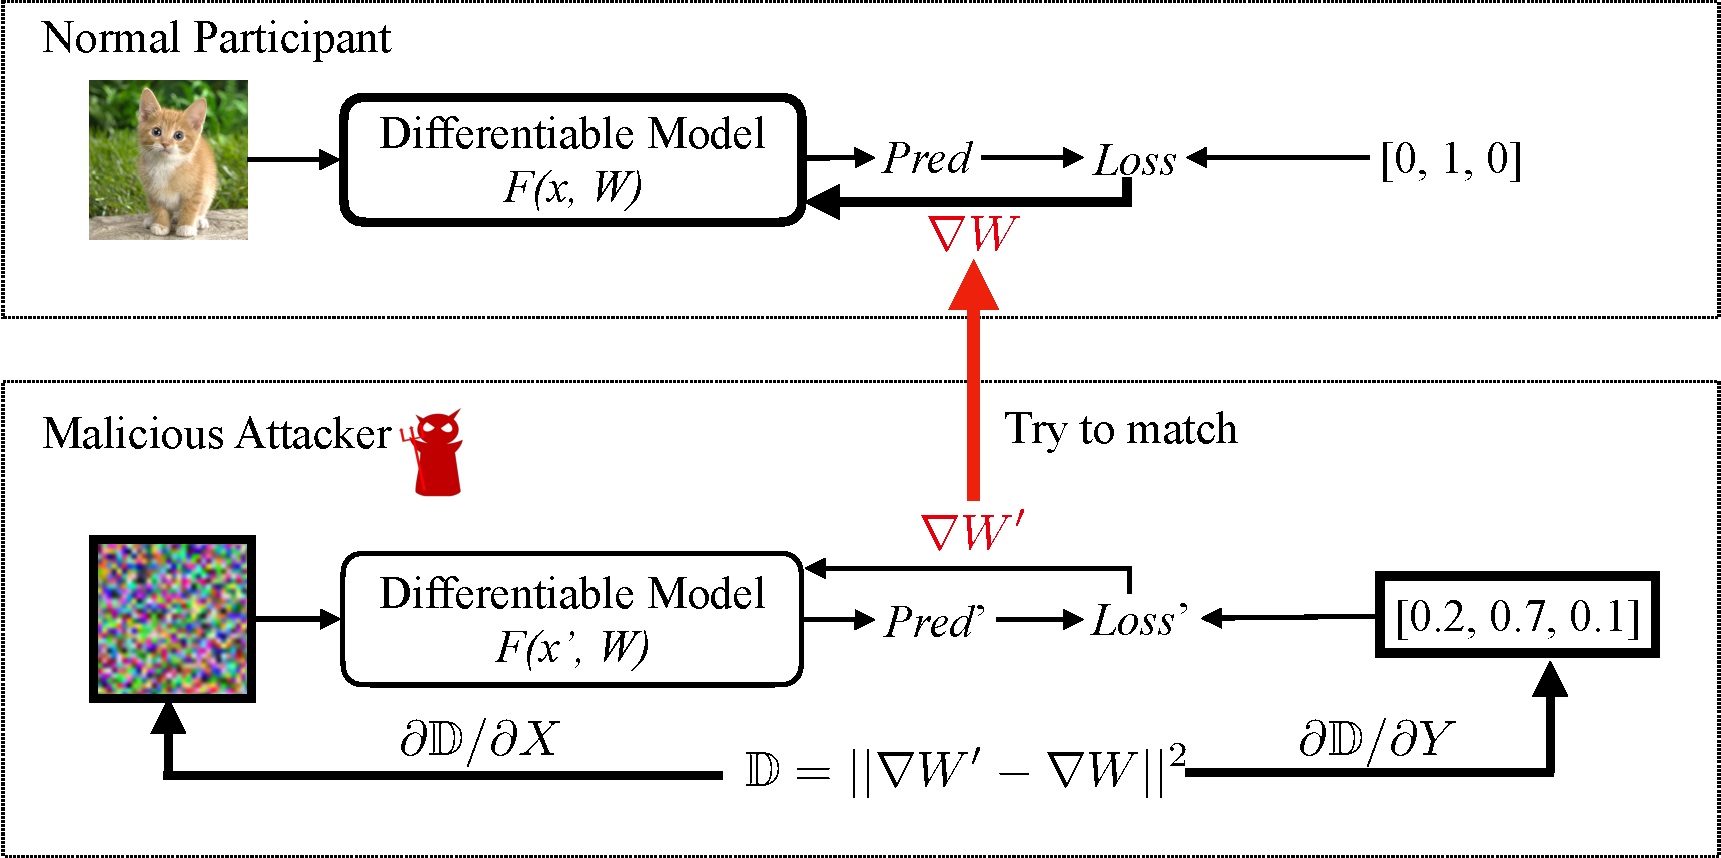
\includegraphics[width=\linewidth]{figures/fig2-crop.pdf}
    \caption{The overview of our DLG algorithm. Variables to be updated are marked with a bold border. While normal participants calculate $\nabla W$ to update parameter using its private training data, the malicious attacker updates its dummy inputs and labels to minimize the gradients distance. When the optimization finishes, the evil user is able to obtain the training set from honest participants.
    }
    \label{fig:methods}
\end{figure}
%%%%%%%%%%%%%%%%%%%%% IN SHORT: Algorithm
% To motivate section, we first describe the problem settings. We then introduce our DLG algorithm and discuss the modification to deal with batched data. 

We show that it's possible to steal an image pixel-wise and steal a sentence token-wise from the gradients. We focus on the standard synchronous distributed training: At each step $t$,  every node $i$ samples a minibatch 
% $(\mathbf{x}_t, \mathbf{y}_t) =  \{ x_{t, j}, y_{t, j} \} _{j=1}^{n} $ 
$(\mathbf{x}_{t, i}, \mathbf{y}_{t, i}) $
from its own dataset to compute the gradients

\begin{equation}
    % \vspace{-10pt}
    \nabla W_{t, i} = \frac{
        \partial \ell (F(\mathbf{x}_{t, i}, W_{t}), \mathbf{y}_{t, i} )
    }{
        \partial W_t
    } 
    % \vspace{-10pt}
\end{equation}

The gradients are averaged across the $N$ servers and then used to update the weights:
\begin{equation}
% \vspace{-10pt}
\begin{split}
    \nabla W_{t} = \frac{1}{N} \sum_{j}^{N}  \nabla W_{t, j}; \quad 
    W_{t+1} = W_{t} - \eta \nabla W_{t}
\end{split}
% \vspace{-10pt}
\end{equation}

% $F()$ and $W_{t}$ are shared by default.
Given gradients $\nabla W_{t, k}$ received from other participant $k$, we aim to steal participant $k$'s training data $(\mathbf{x}_{t, k}, \mathbf{y}_{t, k})$. Note $F()$ and $W_{t}$ are shared by default for synchronized distributed optimization.

% \pagebreak

\subsection{Training Data Leakage through Gradients Matching}\label{sec:algorithm}
\begin{algorithm}[t]
    \caption{Deep Leakage from Gradients.}\label{algorithm:deep_leakage}
    
    \hspace*{\algorithmicindent} \textbf{Input:} 
        $F(\mathbf{x};W)$: Differentiable machine learning model;
        $W$: parameter weights; $\nabla W$: gradients calculated by training data
    \\
    \hspace*{\algorithmicindent} \textbf{Output:} private training data $\mathbf{x}, \mathbf{y}$ 
    \begin{algorithmic}[1]
    \Procedure{DLG}{$F$, $W$, $\nabla W$} % \Comment{The}
        \State $\mathbf{x'}_{1} \gets \mathcal{N}(0, 1)$ 
               , $\mathbf{y'}_{1} \gets \mathcal{N}(0, 1)$ 
        \Comment{Initialize dummy inputs and labels.}
        \For{$i \gets 1 \textrm{ to } n$}
                \State $
                    \nabla W'_i \gets 
                        \partial \ell (F(\mathbf{x'}_i, W_{t}), \mathbf{y'}_i)
                        /
                        \partial W_t
                    $ \Comment{Compute dummy gradients.} 
                \State 
                    $ \mathbb{D}_i \gets ||\nabla W'_i - \nabla W||^2 $ 
                    % \Comment{Compute distance between two gradients.}
                \State 
                    $\mathbf{x}'_{i+1} \gets \mathbf{x}'_i - \eta \nabla_{\mathbf{x}'_i} \mathbb{D}_i$
                   ,
                    $\mathbf{y}'_{i+1} \gets \mathbf{y}'_i - \eta \nabla_{\mathbf{y}'_i} \mathbb{D}_i$
                    \Comment{Update data to match gradients.}
        \EndFor
        \State \textbf{return} $\mathbf{x}'_{n+1}, \mathbf{y}'_{n+1}$
    \EndProcedure
    \end{algorithmic}
\end{algorithm}

To recover the data from gradients, we first randomly initialize a dummy input $\mathbf{x'}$ and label input $\mathbf{y'}$. We then feed these ``dummy data'' into models and get ``dummy gradients''.

\begin{equation}
\nabla W' = \frac{
        \partial \ell (F(\mathbf{x}', W), \mathbf{y}' ) 
    }{
        \partial W
    }
\end{equation}

% As proved in Sec.~\ref{proof}, there is a unique mapping between gradients. In another word, 
Optimizing the dummy gradients close as to original also makes the dummy data close to the real training data (the trends shown in Fig.~\ref{fig:vision_fig3}). Given gradients at a certain step, we obtain the training data by minimizing the following objective 
\begin{align}
\begin{split}
\mathbf{x'}^{*}, \mathbf{y'}^{*}
    = \argmin_{\mathbf{x'}, \mathbf{y}'} ||\nabla W' - \nabla W||^2 
    = \argmin_{\mathbf{x'}, \mathbf{y}'} || 
        \frac{\partial \ell (F(\mathbf{x}', W), \mathbf{y}')}{\partial W} -
        % \frac{\partial \ell (F(\mathbf{x}_t, W_{t}), \mathbf{y}_t)}{\partial W})
        \nabla W
    ||^2
\end{split}
\end{align}

The distance $||\nabla W' - \nabla W||^2$ is differentiable w.r.t dummy inputs $\mathbf{x'}$ and labels $\mathbf{y'}$ can thus can be optimized using standard gradient-based methods. Note that this optimization requires $2^{nd}$ order derivatives. We make a mild assumption that $F$ is twice differentiable, which holds for the majority of modern machine learning models (e.g., most neural networks) and tasks. 

% \pagebreak
% In some tasks, the data may contain discrete parts, e.g., class labels and word vectors. For such a case, we optimize their continuous alternatives instead. More details can be found in the experiment section. 
% 

\subsection{Deep Leakage for Batched Data}\label{sec:algorithm:batched}
% \newcommand\imgwidth{0.080}

\begin{figure}[t]
    \centering
    \begin{tabular}{c c c c c | c | c}
      Iters=0 & Iters=10 & Iters=50 & Iters=100 & Iters=500 & Melis~\cite{Melis2018unintended} & Ground Truth \\
        
\includegraphics[width=\imgwidth\linewidth]{experiments/mnist_0_ours/0000.png} &
        
\includegraphics[width=\imgwidth\linewidth]{experiments/mnist_0_ours/0020.png} &
        
\includegraphics[width=\imgwidth\linewidth]{experiments/mnist_0_ours/0050.png} &
        
\includegraphics[width=\imgwidth\linewidth]{experiments/mnist_0_ours/0100.png} &
        
\includegraphics[width=\imgwidth\linewidth]{experiments/mnist_0_ours/0500.png} &
        
\includegraphics[width=\imgwidth\linewidth]{experiments/mnist_0_others/unintended.png} &
        
\includegraphics[width=\imgwidth\linewidth]{experiments/mnist_0_ours/ground_truth.png} 
      \\ 
        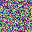
\includegraphics[width=\imgwidth\linewidth]{experiments/cifar100_25_ours/0000.png} &
        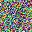
\includegraphics[width=\imgwidth\linewidth]{experiments/cifar100_25_ours/0020.png} &
        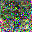
\includegraphics[width=\imgwidth\linewidth]{experiments/cifar100_25_ours/0050.png} &
        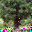
\includegraphics[width=\imgwidth\linewidth]{experiments/cifar100_25_ours/0100.png} &
        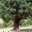
\includegraphics[width=\imgwidth\linewidth]{experiments/cifar100_25_ours/0500.png} &
        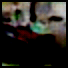
\includegraphics[width=\imgwidth\linewidth]{experiments/cifar100_25_others/unintended.png} &
        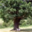
\includegraphics[width=\imgwidth\linewidth]{experiments/cifar100_25_ours/ground_truth.png} 
      \\
        
\includegraphics[width=\imgwidth\linewidth]{experiments/svhn_1_ours/0000.png} &
        
\includegraphics[width=\imgwidth\linewidth]{experiments/svhn_1_ours/0020.png} &
        
\includegraphics[width=\imgwidth\linewidth]{experiments/svhn_1_ours/0050.png} &
        
\includegraphics[width=\imgwidth\linewidth]{experiments/svhn_1_ours/0100.png} &
        
\includegraphics[width=\imgwidth\linewidth]{experiments/svhn_1_ours/0500.png} &
        
\includegraphics[width=\imgwidth\linewidth]{experiments/svhn_1_others/unintended.png} &
        
\includegraphics[width=\imgwidth\linewidth]{experiments/svhn_1_ours/ground_truth.png}
      \\
        
\includegraphics[width=\imgwidth\linewidth]{experiments/lfw_51_ours/0000.png} &
        
\includegraphics[width=\imgwidth\linewidth]{experiments/lfw_51_ours/0020.png} &
        
\includegraphics[width=\imgwidth\linewidth]{experiments/lfw_51_ours/0050.png} &
        
\includegraphics[width=\imgwidth\linewidth]{experiments/lfw_51_ours/0100.png} &
        
\includegraphics[width=\imgwidth\linewidth]{experiments/lfw_51_ours/0500.png} &
        
\includegraphics[width=\imgwidth\linewidth]{experiments/lfw_51_others/unintended.png} &
        
\includegraphics[width=\imgwidth\linewidth]{experiments/lfw_51_ours/ground_truth.png}
      \\
    \end{tabular}
    \caption{The visualization showing the deep leakage on images from MNIST~\cite{lecun1998mnist}, CIFAR-100~\cite{krizhevsky2009cifar}, SVHN~\cite{netzer2011svhn} and LFW~\cite{LFWTech} respectively. 
    Our algorithm fully recovers the four images while previous work only succeeds on simple images with clean backgrounds.
    % More examples can be found in appendix. \zhijian{I think one visualization for the history should be enough; we can put more final results}
    }
    \label{fig:experiment_vision}
\end{figure}


The algo.~\ref{algorithm:deep_leakage} works well when there is only a single pair of input and label in the batch. However when we naively apply it to the case where batch size $N \ge 1$, the algorithm would be too slow to converge. We think the reason is that batched data can have $N!$ different permutations and thus make optimizer hard to choose gradient directions. 
% 
To force the optimization closer to a solution, instead of updating the whole batch, we update a single training sample instead. 
%
We modify the \textit{line 6} in algo.~\ref{algorithm:deep_leakage} to : 

\begin{align}
\begin{split}
    \mathbf{x'}^{i \bmod N}_{t+1} &\leftarrow \mathbf{x'}^{i \bmod N}_{t} - \nabla_{\mathbf{x'}^{i \bmod N}_{t+1}} \mathbb{D}
    \\
    \mathbf{y'}^{i \bmod N}_{t+1} &\leftarrow \mathbf{y'}^{i \bmod N}_{t} - \nabla_{\mathbf{y'}^{i \bmod N}_{t+1}} \mathbb{D}
\end{split}
\end{align}

Then we can observe fast and stable convergence. We list the iterations required for convergence for different batch sizes in Tab.~\ref{tab:batched_restore} and provide visualized results in Fig.~\ref{fig:experiment_vision_multi_batch}. The larger the batch size is, the more iterations DLG requires to attack. 

\begin{table}[h]
    \centering
    \begin{tabular}{c|c|c|c|c}
                  & BS=1 & BS=2 & BS=4 & BS=8 \\ \hline
        ResNet-20 & 270 & 602 & 1173 & 2711 
    \end{tabular}
    \caption{The iterations required for restore batched data on CIFAR~\cite{krizhevsky2009cifar} dataset. 
    }
    \label{tab:batched_restore}
\end{table}
\newcommand{\bigcell}[2]{
    \begin{tabular}{@{}#1@{}}
        #2
    \end{tabular}
}

\begin{figure}[b]
    \centering
    \small
    \begin{tabular}{c c c c c c c c c c}
      % Iters=0 & Iters=10 & Iters=50 & Iters=100 & Iters=500 & Melis~\cite{Melis2018unintended} & Ground Truth \\
        Initial     &
        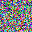
\includegraphics[width=\imgwidth\linewidth]{experiments/multi_batch/0-0.png} &
        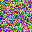
\includegraphics[width=\imgwidth\linewidth]{experiments/multi_batch/1-0.png} &
        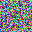
\includegraphics[width=\imgwidth\linewidth]{experiments/multi_batch/2-0.png} &
        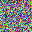
\includegraphics[width=\imgwidth\linewidth]{experiments/multi_batch/3-0.png} &
        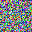
\includegraphics[width=\imgwidth\linewidth]{experiments/multi_batch/4-0.png} &
        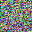
\includegraphics[width=\imgwidth\linewidth]{experiments/multi_batch/5-0.png} &
        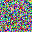
\includegraphics[width=\imgwidth\linewidth]{experiments/multi_batch/6-0.png} &
        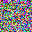
\includegraphics[width=\imgwidth\linewidth]{experiments/multi_batch/7-0.png} 
      \\ 
        Middle Stage   &
        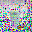
\includegraphics[width=\imgwidth\linewidth]{experiments/multi_batch/0-100.png} &
        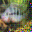
\includegraphics[width=\imgwidth\linewidth]{experiments/multi_batch/1-100.png} &
        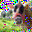
\includegraphics[width=\imgwidth\linewidth]{experiments/multi_batch/2-100.png} &
        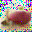
\includegraphics[width=\imgwidth\linewidth]{experiments/multi_batch/3-100.png} &
        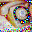
\includegraphics[width=\imgwidth\linewidth]{experiments/multi_batch/4-100.png} &
        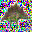
\includegraphics[width=\imgwidth\linewidth]{experiments/multi_batch/5-100.png} &
        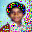
\includegraphics[width=\imgwidth\linewidth]{experiments/multi_batch/6-100.png} &
        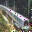
\includegraphics[width=\imgwidth\linewidth]{experiments/multi_batch/7-100.png} 
      \\
        Fully  Leaked &
        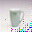
\includegraphics[width=\imgwidth\linewidth]{experiments/multi_batch/0-400.png} &
        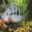
\includegraphics[width=\imgwidth\linewidth]{experiments/multi_batch/1-400.png} &
        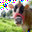
\includegraphics[width=\imgwidth\linewidth]{experiments/multi_batch/2-400.png} &
        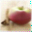
\includegraphics[width=\imgwidth\linewidth]{experiments/multi_batch/3-400.png} &
        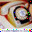
\includegraphics[width=\imgwidth\linewidth]{experiments/multi_batch/4-400.png} &
        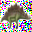
\includegraphics[width=\imgwidth\linewidth]{experiments/multi_batch/5-400.png} &
        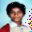
\includegraphics[width=\imgwidth\linewidth]{experiments/multi_batch/6-400.png} &
        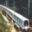
\includegraphics[width=\imgwidth\linewidth]{experiments/multi_batch/7-400.png} 
      \\ % \hline
        Ground  Truth &
        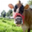
\includegraphics[width=\imgwidth\linewidth]{experiments/multi_batch/0-ground-truth.png} &
        
\includegraphics[width=\imgwidth\linewidth]{experiments/multi_batch/1-ground-truth.png} &
        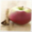
\includegraphics[width=\imgwidth\linewidth]{experiments/multi_batch/2-ground-truth.png} &
        
\includegraphics[width=\imgwidth\linewidth]{experiments/multi_batch/3-ground-truth.png} &
        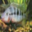
\includegraphics[width=\imgwidth\linewidth]{experiments/multi_batch/4-ground-truth.png} &
        
\includegraphics[width=\imgwidth\linewidth]{experiments/multi_batch/5-ground-truth.png} &
        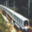
\includegraphics[width=\imgwidth\linewidth]{experiments/multi_batch/6-ground-truth.png} &
        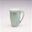
\includegraphics[width=\imgwidth\linewidth]{experiments/multi_batch/7-ground-truth.png} 
      \\
    \end{tabular}
    \caption{Results of deep leakage of batched data. Though the order may not be the same and there are more artifact pixels, DLG still produces images very close to the original ones.}
    \label{fig:experiment_vision_multi_batch}
    \vspace{-10pt}
\end{figure}
\pagebreak
